%%
% This is an Overleaf template for scientific articles and reports
% using the TUM Corporate Design https://www.tum.de/cd
%
% For further details on how to use the template, take a look at our
% GitLab repository and browse through our test documents
% https://gitlab.lrz.de/latex4ei/tum-templates.
%
% The tumarticle class is based on the KOMA-Script class scrartcl.
% If you need further customization please consult the KOMA-Script guide
% https://ctan.org/pkg/koma-script.
% Additional class options are passed down to the base class.
%
% If you encounter any bugs or undesired behaviour, please raise an issue
% in our GitLab repository
% https://gitlab.lrz.de/latex4ei/tum-templates/issues
% and provide a description and minimal working example of your problem.
%%

\documentclass[
  english,        % define the document language (english, german)
  font=times,     % define main text font (helvet, times, palatino, libertine)
  twocolumn,      % use onecolumn or twocolumn layout
]{tumarticle}

\usepackage{cite}

% Add packages here:
\usepackage{booktabs}
\usepackage{siunitx}
\sisetup{group-separator={,}, group-minimum-digits=4}

% article metadata
\title{First Assignment - Business Process Prediction, Simulation, and Optimization - Summer Semester 2026}
\subtitle{Process and Data Science on the BPIC-17 Event Log}

\author[email=lars.heimann@tum.de]{Lars Heimann}

\date\today

\begin{document}

\maketitle

\begin{abstract}
The BPIC-17 dataset records loan applications at a Dutch financial institute. This report systematically extracts, evaluates, and refines a process model from these logs. Basic and advanced event statistics expose process complexity, driving the selection of an Inductive Miner model after evaluating precision-fitness trade-offs. The resulting model serves as a robust foundation for simulation, supplemented by concept drift analysis across quarters to highlight shifting behavior.
\end{abstract}
%

\section{Introduction}
% Write a brief introduction to your report based on ex-
% ternal sources and your own findings. Describe the
% event log: its application domain, when and why it
% was generated, and what business process it captures.
In this report, the dataset BPIC-17 \cite{BPI_data} is analyzed focusing on the systematic creation of a process model and its evaluation. The data was generated by a Dutch financial institute and consists of all applications from 2016 and their processing until February 2nd 2017 \cite{BPIC_2017challenge}. It was provided as part of a competition in 2017 where teams from academia, professional and student teams competed against each other \cite{BPIC_2017challenge}. The event log captures the loan application process, including application processing, offer generation and fraud detection. One notable achievement from this competition was an AS-IS model with a fitness of 97.28\% and a precision of 98.72\% while maintaining fitness by the academic team Rodriques et al. in 2017 \cite{rodrigues2017academics}.

\section{Approach and Results}
Lorem ipsum dolor sit amet, consectetur adipiscing elit, sed do eiusmod tempor 
incididunt ut labore et dolore magna aliqua. Ut enim ad minim veniam, quis 
nostrud exercitation ullamco laboris nisi ut aliquip ex ea commodo consequat. 
Duis aute irure dolor in reprehenderit in voluptate velit esse cillum dolore 
eu fugiat nulla pariatur. Excepteur sint occaecat cupidatat non proident, sunt 
in culpa qui officia deserunt mollit anim id est laborum.

\subsection{Technical Setup and Preliminaries}
% Describe your technical setup: Python libraries used,
% visualization techniques, and process modeling tools.
% Provide a footnote for each package, library, and tool.

The technical setup used for this assignment consists of Python \footnote{\tiny Python \url{https://www.python.org}} in conjunction with various dependencies. Most data handling was done using numpy \footnote{\tiny NumPy \url{https://numpy.org}} and pandas \footnote{\tiny pandas \url{https://pandas.pydata.org}}, visualization were created using seaborn \footnote{\tiny seaborn \url{https://seaborn.pydata.org}} and matplotlib \footnote{\tiny matplotlib \url{https://matplotlib.org}}. For process modeling, pm4py \footnote{\tiny pm4py \url{https://processintelligence.solutions/pm4py}} was primarily used. Machine learning was handled through scikit-learn \footnote{\tiny scikit-learn \url{https://scikit-learn.org/stable}}.

% Example footnote: 
% Python \footnote{\tiny Python \url{https://www.python.org}}

\subsection{Basic Analysis}
To get a general understanding of the process, Table~\ref{tab:statistics} presents the key metrics. The event log covers \num{31509} cases across roughly \num{1.2} million events, providing a solid base for process mining. On average, a case consists of \num{38.16} events spread across \num{21.9} days. Both statistics have very high standard deviations ($\sigma_{\text{len}}=16.72$ events, $\sigma_{\text{dur}}=13.17$ days), suggesting large process variability. Of the \num{15} event attributes, \num{6} are categorical (non-numeric, non-temporal, $\le 50$ distinct values). This threshold deliberately excludes \texttt{org:resource} with \num{149} unique employees and identifier columns such as \texttt{EventID} (see Section~\ref{sec:addstats}). The minimum number of events recorded for a case was \num{10} and the maximum \num{180}, further corroborating the large variance in case length. The distributions of case length and duration are shown in Figure~\ref{fig:distributions} (Appendix~\ref{sec:appendix}).

\begin{table}[h]
    \caption{Basic event log statistics for BPIC-17. Rows above the rule are the assignment-mandated metrics; rows below are the additional statistics of choice (see Section~\ref{sec:addstats}).}
    \centering
    \footnotesize
    \renewcommand{\arraystretch}{1.00}
    \setlength{\tabcolsep}{4pt}
    \begin{tabular}{lr}
        \toprule
        \textbf{Metric} & \textbf{Value} \\
        \midrule
        No.\ of cases                           & \num{31509}          \\
        No.\ of events                          & \num{1202267}        \\
        No.\ of process variants                & \num{15930}          \\
        No.\ of case attributes                 & \num{4}              \\
        No.\ of event attributes                & \num{15}             \\
        No.\ of categorical event attrs.        & \num{6}              \\
        Mean case length (events)               & \num{38.16}          \\
        $\sigma$ case length (events)           & \num{16.72}          \\
        Mean case duration (days)               & \num{21.90}          \\
        $\sigma$ case duration (days)           & \num{13.17}          \\
        \midrule
        Distinct activities                     & \num{26}             \\
        Median case duration (days)             & \num{19.09}          \\
        Min case length (events)                & \num{10}             \\
        Max case length (events)                & \num{180}            \\
        Distinct resources                      & \num{149}            \\
        Distinct start activities               & \num{1}              \\
        Distinct end activities                 & \num{12}             \\
        \bottomrule
    \end{tabular}
    \label{tab:statistics}
\end{table}

\subsubsection*{Additional statistics of choice}\label{sec:addstats}
The assignment requires at least two extra statistics. We report five additional statistics to capture process details not covered by the mandated metrics:
\begin{itemize}
    \item \textbf{Distinct activities} (\num{26}): sets the upper bound on model complexity.
    \item \textbf{Median case duration} (\num{19.09} days vs.\ mean \num{21.90}): complements the mean because the duration distribution is right-skewed. A median below the mean confirms the skew and motivates non-parametric tests in Section~\ref{sec:advanced}.
    \item \textbf{Min / max case length} (\num{10} / \num{180}): shows a significant spread between the extremes. The large difference indicates that a single standard path cannot adequately capture all cases.
    \item \textbf{Distinct resources} (\num{149}): we exclude \texttt{org:resource} from the categorical-attribute count for this reason; it is reported separately because it sizes the workforce and forms the basis for resource simulation.
    \item \textbf{Distinct start / end activities} (\num{1} / \num{12}): indicates a single entry point (\texttt{A\_Create\_Application}) and twelve distinct termination activities, showing the process is funnel-shaped on entry and branched on exit. This is relevant when choosing initial and final markings for the Petri net.
\end{itemize}

Activity frequencies and the temporal distribution of events are shown in Figures~\ref{fig:activities} and~\ref{fig:events-time} in Appendix~\ref{sec:appendix}.

\subsection{Process Model Creation and Validation}\label{sec:model}

Before discovery the log is filtered to events with \texttt{lifecycle:transition\,=\,complete}. The BPIC-17 log records up to seven lifecycle transitions per activity (\texttt{schedule}, \texttt{start}, \texttt{complete}, \texttt{ate\_abort}, \texttt{withdraw}, \texttt{suspend}, \texttt{resume}); keeping all of them would make each user-facing step contribute multiple events and the discovered net would carry a spurious self-loop on essentially every activity. After filtering we retain all \num{31509} cases over \num{475306} events covering \num{24} of the \num{26} distinct activities; the two work activities that never reach the \texttt{complete} stage (\mbox{\texttt{W\_Personal Loan collection}} and \mbox{\texttt{W\_Shortened completion}}) drop out of discovery and are not represented in any of the discovered models. On this input we apply three discovery algorithms, evaluate them against the four standard quality dimensions plus two custom simplicity metrics, iteratively refine the most suitable algorithm into a final model, and perform decision mining on every XOR gateway in that model.

We apply three discovery algorithms covering two algorithmic families. The Inductive Miner (IM)~\cite{leemans2013inductive} recursively splits the log into sequence, exclusive choice, parallel, and loop blocks and returns a sound workflow net with fitness equal to one. Its infrequent variant (IMf)~\cite{leemans2014infrequent} adds a noise threshold that prunes infrequent directly-follows edges before the cut detection, trading fitness for precision and simplicity. The Heuristics Miner (HM)~\cite{weijters2006heuristics} is a frequency-based method that constructs the net edge by edge from the directly-follows graph; it tolerates noise well but does not guarantee soundness, which matters for the downstream use of the model as a simulation skeleton. We exclude the Alpha Miner because BPIC-17 contains loops that Alpha cannot represent. The two custom simplicity metrics reported next to the standard PM4Py score are the coefficient of network connectivity~\cite{carmona2018conformance} normalised as $1/(1+|F|/(|P|+|T|))$ and the inverse mean place degree $1/(1+\bar d_p)$ with $d_p = |\mathit{in}(p)| + |\mathit{out}(p)|$; both put simpler models closer to one.

Table~\ref{tab:models} reports the quality of the three discovered models on the lifecycle-filtered log. IM perfectly replays the log but allows almost any sequence of activities, which shows in its precision of $0.293$ (classical flower behaviour). The infrequent variant at the default noise threshold of $0.2$ filters part of the rare paths and lifts precision to $0.339$ at a fitness cost of less than one percent, while shrinking the net from 34 to 30 places. Heuristics Miner sits at the opposite end of the trade-off: its $0.998$ precision is the highest by a wide margin, but fitness drops to $0.836$ and the net is about twice the size of either Inductive Miner output (220 arcs against 102 to 114). On simplicity all three sit in a comparable band on the PM4Py and CNC scales, with HM scoring slightly lower because of its higher arc count.

\begin{table}[h]
    \caption{Quality of the three discovered models on the lifecycle-filtered log. Higher is better for every metric except $|P|$, $|T|$, $|F|$.}
    \centering
    \footnotesize
    \setlength{\tabcolsep}{4pt}
    \begin{tabular}{lrrr}
        \toprule
        \textbf{Metric}             & \textbf{IM} & \textbf{HM} & \textbf{IMf}\,(0.2) \\
        \midrule
        Fitness (log)               & 1.000 & 0.836 & 0.994 \\
        Precision                   & 0.293 & 0.998 & 0.339 \\
        Generalization              & 0.976 & 0.828 & 0.981 \\
        Simplicity (PM4Py)          & 0.617 & 0.481 & 0.632 \\
        Simplicity (CNC)            & 0.433 & 0.394 & 0.436 \\
        Simplicity (place degree)   & 0.230 & 0.182 & 0.227 \\
        \midrule
        $|P|$ / $|T|$ / $|F|$       & 34/53/114 & 49/94/220 & 30/49/102 \\
        \bottomrule
    \end{tabular}
    \label{tab:models}
\end{table}

We select the Inductive Miner infrequent model as the foundation for the final process. Since the model will be used in a process simulator, soundness is strictly required to prevent deadlocks and ensure proper termination. IM and IMf inherently guarantee this, whereas HM does not. Additionally, the infrequent variant's noise threshold allows a systematic trade-off between fitness, precision, and simplicity.

\subsubsection*{Threshold selection}\label{sec:sweep}

The noise threshold of IMf prunes directly-follows edges below a given relative frequency before the recursive cut detection. Higher thresholds remove more rare behaviour, which lifts precision and simplicity at the expense of fitness. The threshold was first swept over $\{0.0, 0.05, 0.1, 0.15, 0.2, 0.3, 0.4, 0.5\}$. Fitness barely moved across this range (it stayed above $0.95$ everywhere) while precision was flat at roughly $0.34$ up to threshold $0.4$ and then jumped to $0.574$ at threshold $0.5$. The first natural pick was threshold $0.5$.

Because the cliff between $0.4$ and $0.5$ was unexpected and the upper half of the threshold range had not been tested, the sweep was extended with $\{0.6, 0.7, 0.8, 0.9, 0.95\}$. A second cliff appears between $0.8$ and $0.9$: precision jumps from $0.556$ to $\mathbf{0.711}$, fitness loses one percentage point ($0.874 \to 0.863$), and simplicity stays at $0.684$. The full sweep is shown in Figure~\ref{fig:sweep} (Appendix~\ref{sec:appendix}). The threshold $0.9$ model dominates the $0.5$ candidate on precision while keeping fitness comfortably above the $0.8$ target set in the assignment, so it is adopted as the final model.

A limitation of this approach is that precision and simplicity cannot be pushed above $0.8$ simultaneously. At a threshold of $0.95$, simplicity peaks at $0.684$ and precision at $0.711$. Therefore, we prioritize meeting the fitness constraint, accepting the asymptotic limits of the other metrics as a structural characteristic of the log.

We prioritize precision, simplicity, and generalization over maximum fitness. A model with perfect fitness but very low precision allows almost any sequence of activities, leading to simulated traces that do not resemble real behavior. In contrast, a precise and sound model with an $86\%$ fitness serves as a much more reliable basis for resource scheduling and waiting-time analysis.

After discovering the process model, decision mining is applied to the XOR splits to find out if case attributes can explain the routing choices. The final net contains five XOR splits, two of which have labeled outgoing transitions. We evaluated attributes such as \texttt{LoanGoal}, \texttt{ApplicationType}, and \texttt{RequestedAmount} using decision tree classifiers with a maximum depth of 4. For both viable XOR splits, the test accuracy matched the majority-class base rate. The attributes carry no predictive signal for the routing decisions. This suggests that routing depends heavily on event-level data acquired during execution rather than static case attributes.

The discovered process model is shown as BPMN~2.0 in Figure~\ref{fig:bpmn} (Appendix~\ref{sec:appendix}).

\subsection{Advanced Analysis: Concept Drift Detection}\label{sec:advanced}
We hypothesize that the loan application process exhibits concept drift over time, meaning the distribution of process behavior shifts between the quarters of 2016. Analyzing this drift is highly relevant for process simulation, as a model configured with data from the entire year may inaccurately predict performance in a subsequent period if the underlying dynamics have changed.

We approach this by splitting the log into four quarters and performing statistical tests on key process dimensions. First, a Kruskal-Wallis test on case durations yields an H-statistic of $167.39$ ($p < 0.001$), confirming a significant shift in processing times across quarters. Second, a Chi-squared test comparing the activity distributions between the first and fourth quarters results in a $\chi^2$ value of $524.26$ ($p < 0.001$), demonstrating that the relative frequencies of activities performed also change significantly. Lastly, another Kruskal-Wallis test reveals significant drift in the requested loan amounts ($H = 228.81, p < 0.001$). The visual evidence for these shifts is provided in Figures~\ref{fig:drift_durations}, \ref{fig:drift_activities}, and \ref{fig:drift_amounts} (Appendix~\ref{sec:appendix}). 

These findings have direct implications for simulation design. The significant drift in case durations and activity frequencies suggests that a stationary simulation model is inadequate. To accurately simulate future states, the model's parameters should be calibrated using the most recent time window or a rolling window approach, rather than averaging historical data that no longer reflects the current process reality.

\section*{Usage Declaration: AI tools}
Claude Code\footnote{\tiny Claude Code \url{https://www.anthropic.com/claude-code}} using Opus 4.7\footnote{\tiny Opus 4.7 \url{https://www.anthropic.com/claude/opus}} was used during the preparation of this report. Specifically, it assisted with ideation, preliminary exploratory data analysis, and the formulation of report passages. It was further used for help with \LaTeX{} formatting (table layout, figure placement, appendix structure) and for refactoring the analysis code (consolidating statistics into a single computation, removing duplication). All analytical decisions, interpretations and final wording are my responsibility.


\onecolumn
\bibliographystyle{plain}
\bibliography{references}

\appendix
\section{Figures}\label{sec:appendix}

\begin{figure}[h]
    \centering
    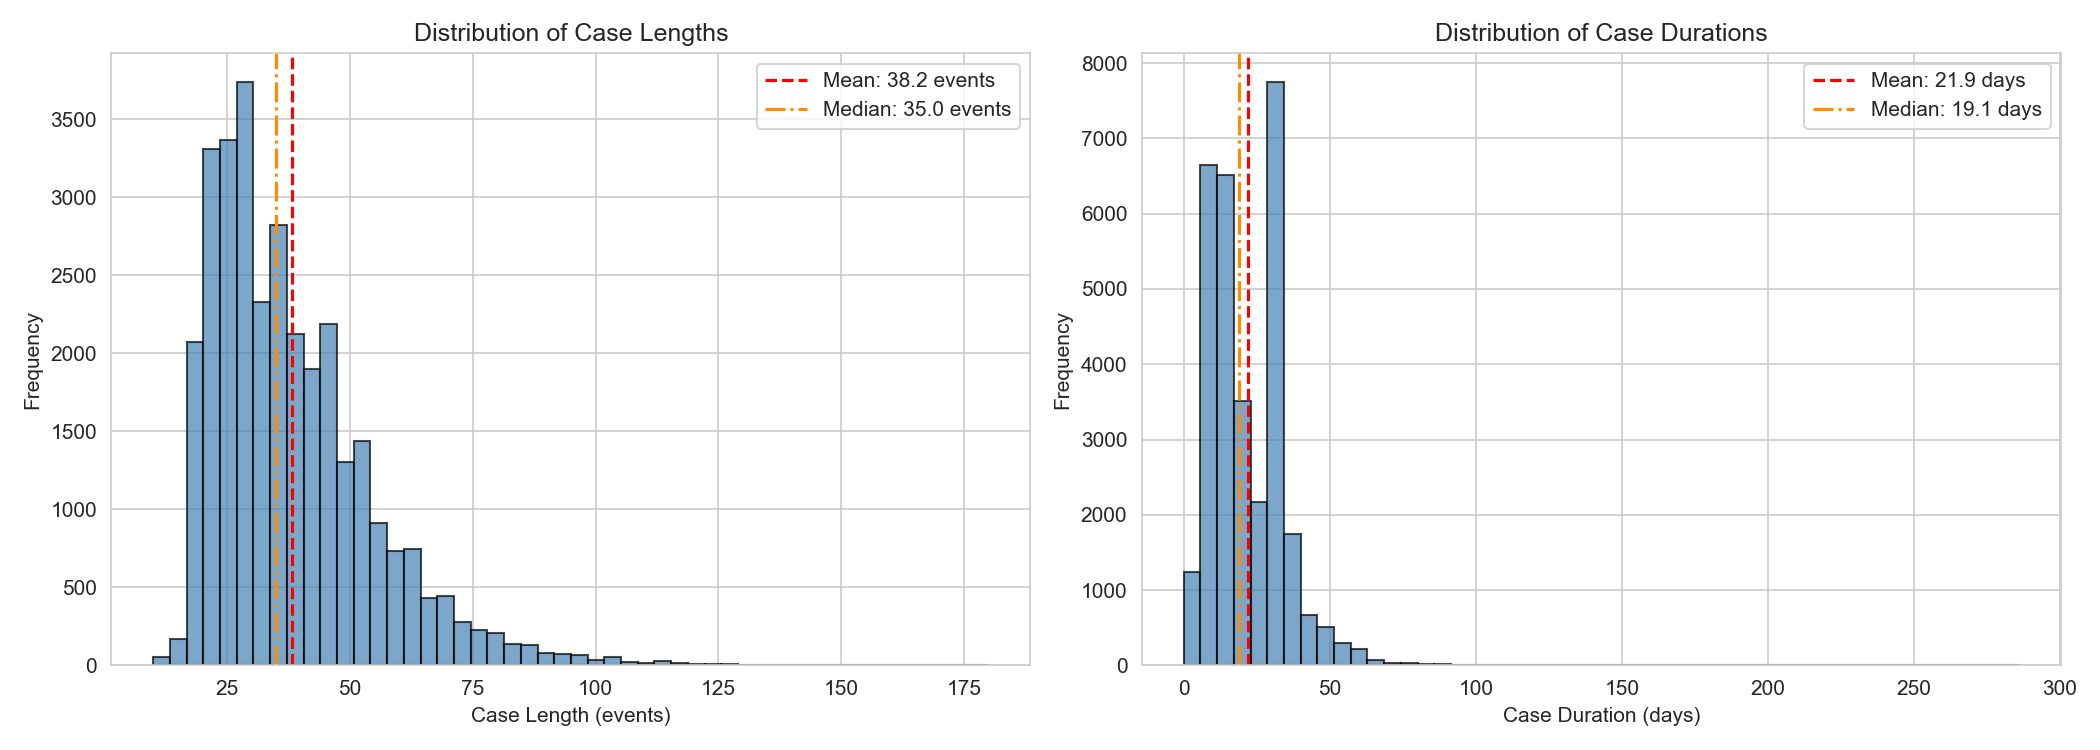
\includegraphics[width=\textwidth]{figures/distributions.png}
    \caption{Distributions of case length in no. of events (left) and case duration in days (right). Both are right-skewed, with a long tail of cases that are much longer than the mean. Case length is a lot more skewed than case duration. The red dashed line marks the mean, the orange dash-dotted line the median.}
    \label{fig:distributions}
\end{figure}

\begin{figure}[h]
    \centering
    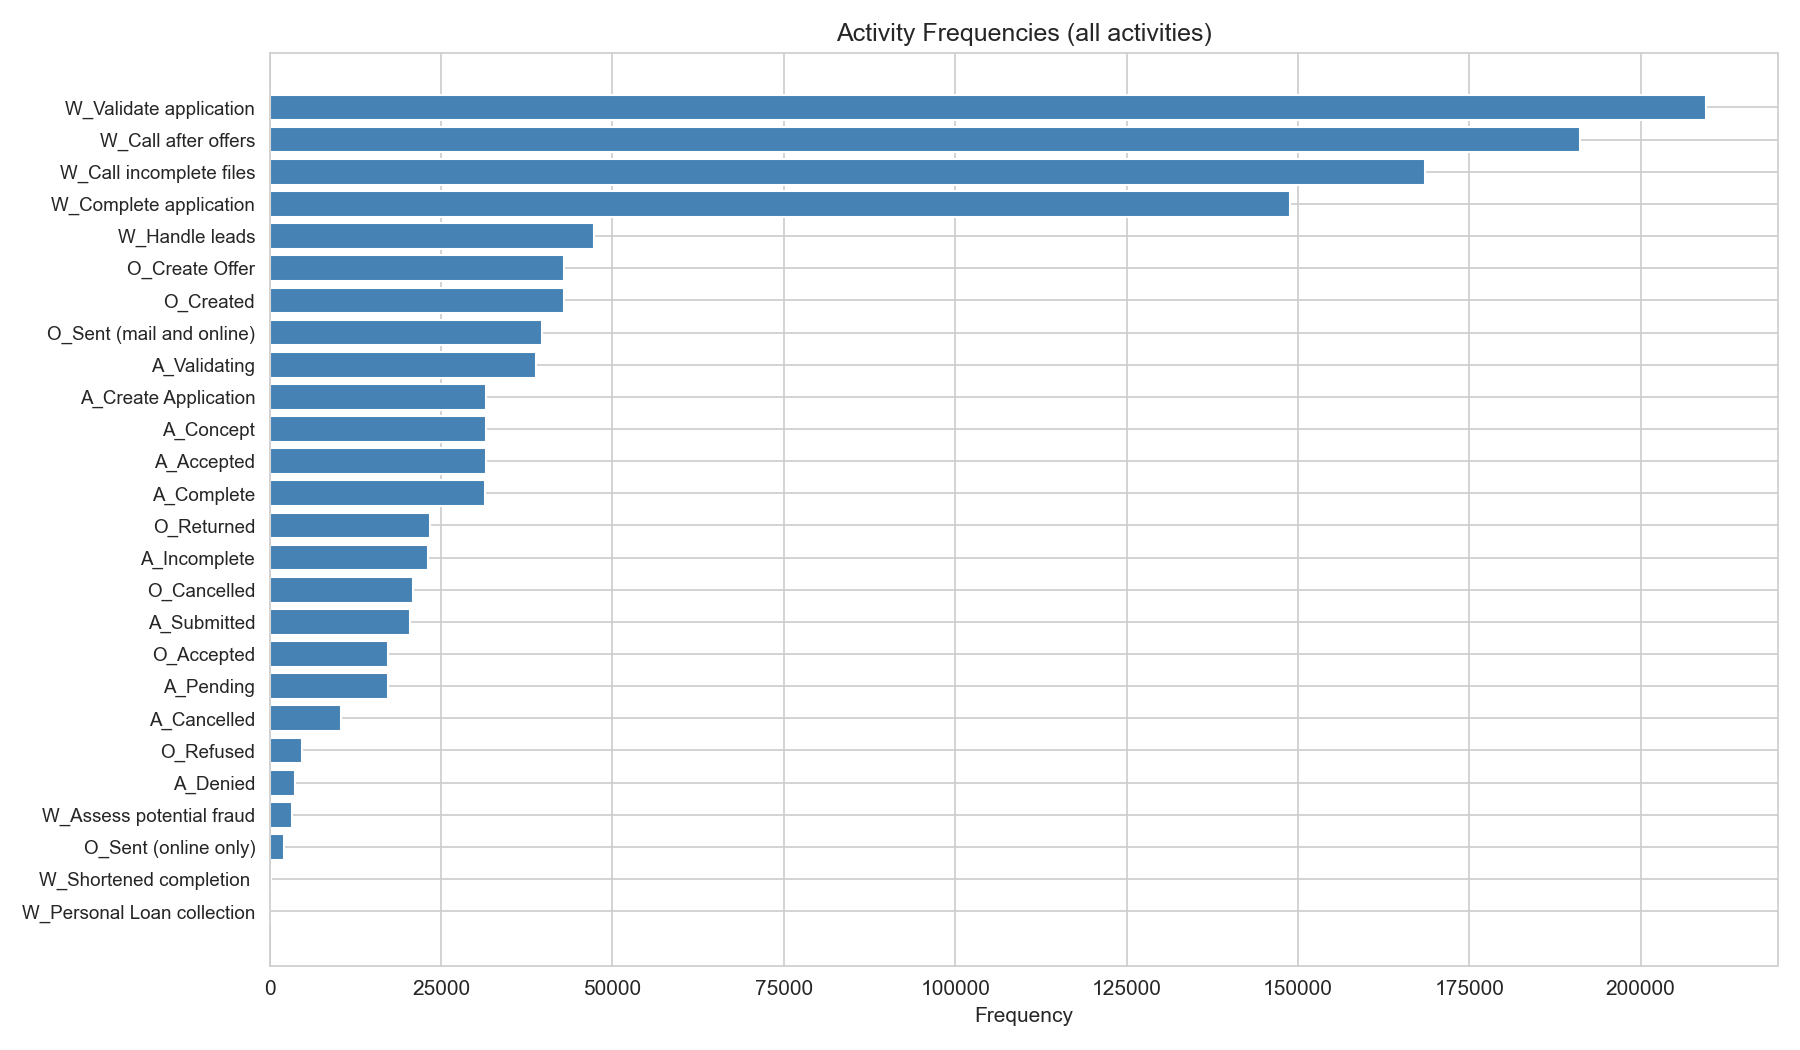
\includegraphics[width=\textwidth]{figures/activity_frequencies.png}
    \caption{Activity frequencies across all \num{1202267} events. The top four activities (\texttt{W\_Validate application}, \texttt{W\_Call after offers}, \texttt{W\_Call incomplete files}, \texttt{W\_Complete application}) dominate, making up \num{718017} (\SI{59.72}{\percent}) of the total 1.2 million events.}
    \label{fig:activities}
\end{figure}

\begin{figure}[h]
    \centering
    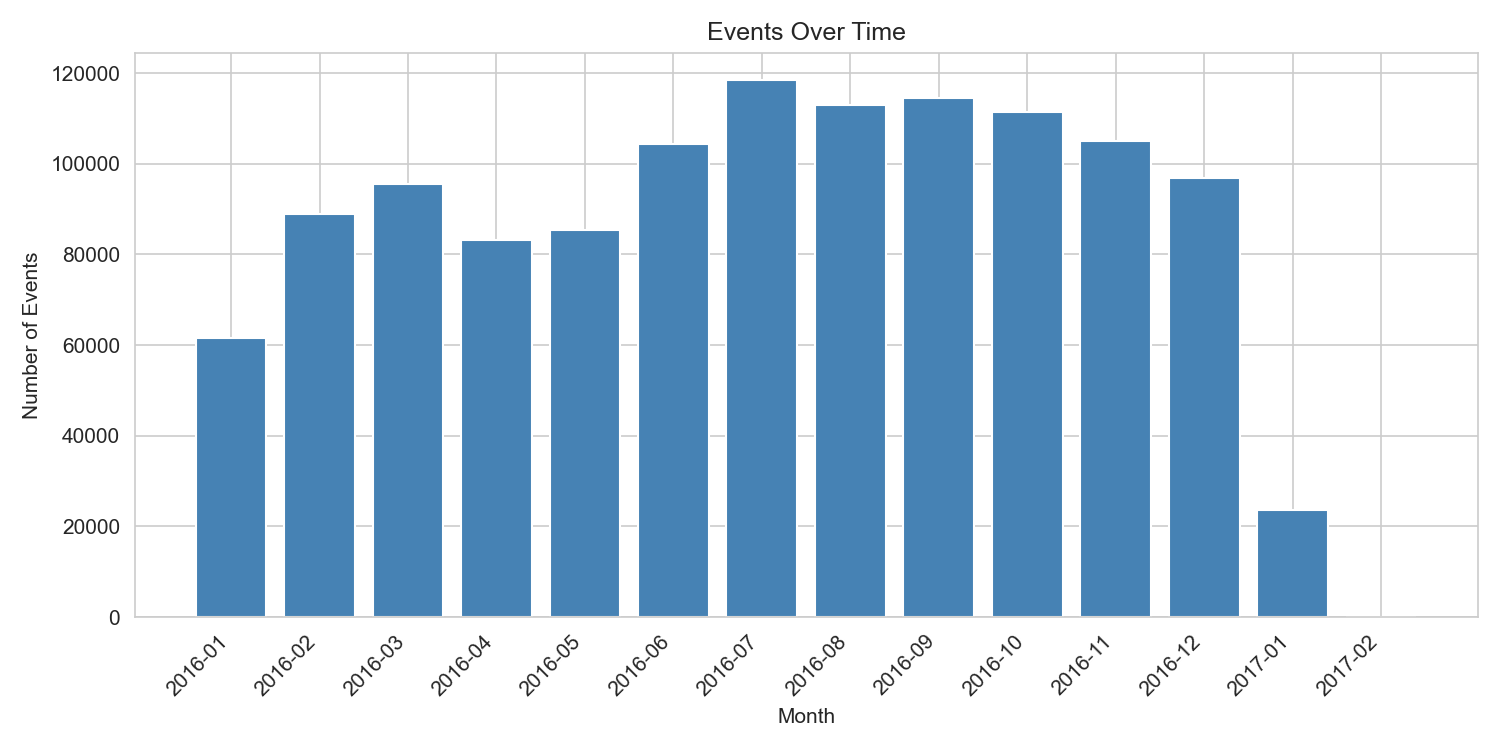
\includegraphics[width=\textwidth]{figures/events_over_time.png}
    \caption{Number of events per calendar month over the observation window of the BPIC-17 event log. Volume rises sharply from the first weeks of 2016 and stabilises around the spring; the partial drop in early 2017 reflects the cut-off of the extraction window on February 2nd 2017.}
    \label{fig:events-time}
\end{figure}

\begin{figure}[h]
    \centering
    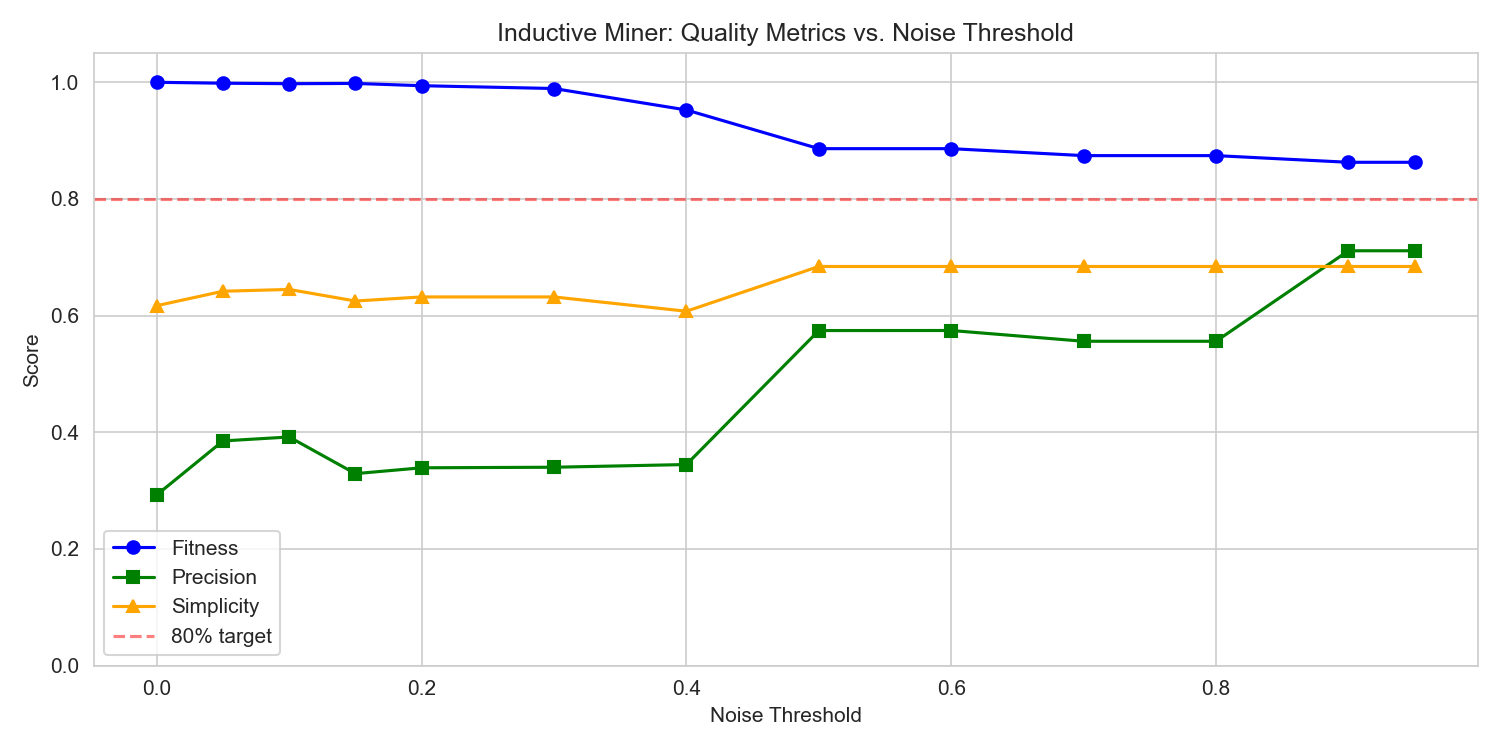
\includegraphics[width=\textwidth]{figures/threshold_sweep.png}
    \caption{Inductive Miner infrequent: fitness, precision, and PM4Py simplicity as a function of the noise threshold. Two precision cliffs appear, one between $0.4$ and $0.5$ and a second between $0.8$ and $0.9$. Fitness stays above the $0.8$ target across the whole sweep. The chosen threshold is $0.9$ (see Section~\ref{sec:sweep}).}
    \label{fig:sweep}
\end{figure}

\begin{figure}[h]
    \centering
    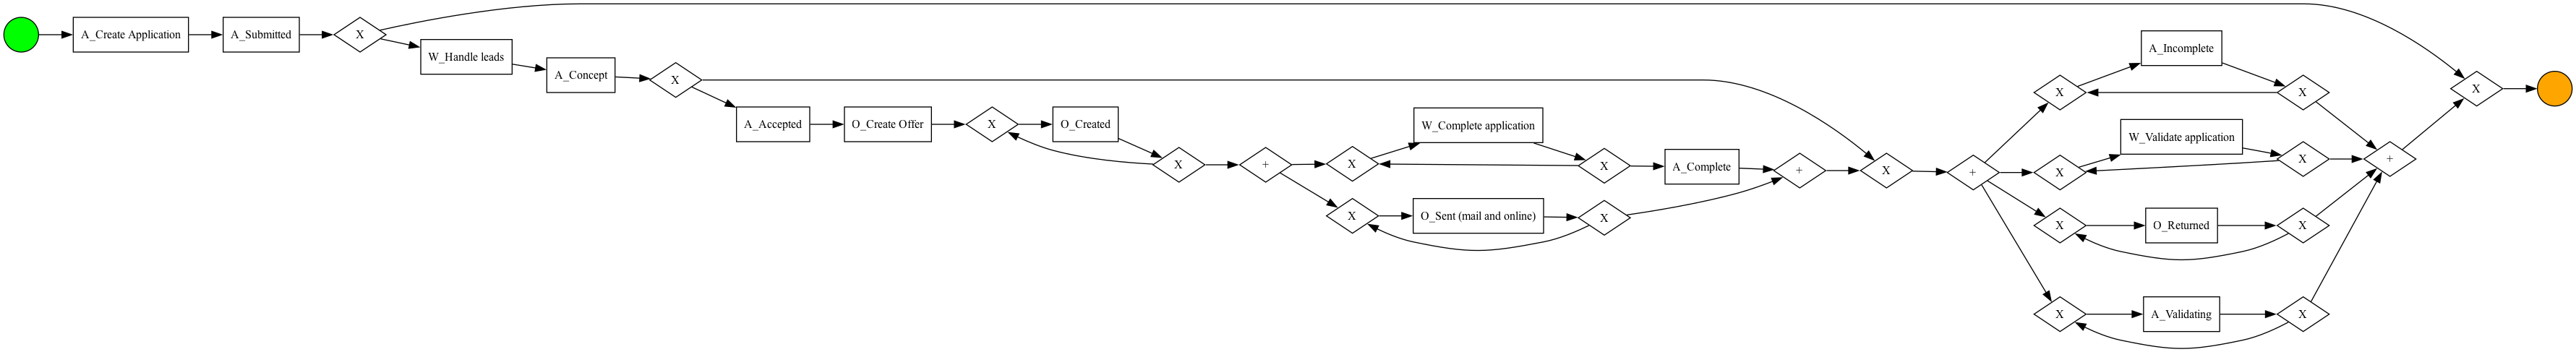
\includegraphics[width=\textwidth]{figures/final_bpmn.png}
    \caption{Final process model as BPMN~2.0, discovered with Inductive Miner infrequent at noise threshold $0.9$ on the lifecycle-filtered log. Sound by construction (no deadlocks, proper termination). Fitness $0.863$, precision $0.711$, generalization $0.850$, simplicity (PM4Py) $0.684$; $24$ places, $28$ transitions, $64$ arcs.}
    \label{fig:bpmn}
\end{figure}

\begin{figure}[h]
    \centering
    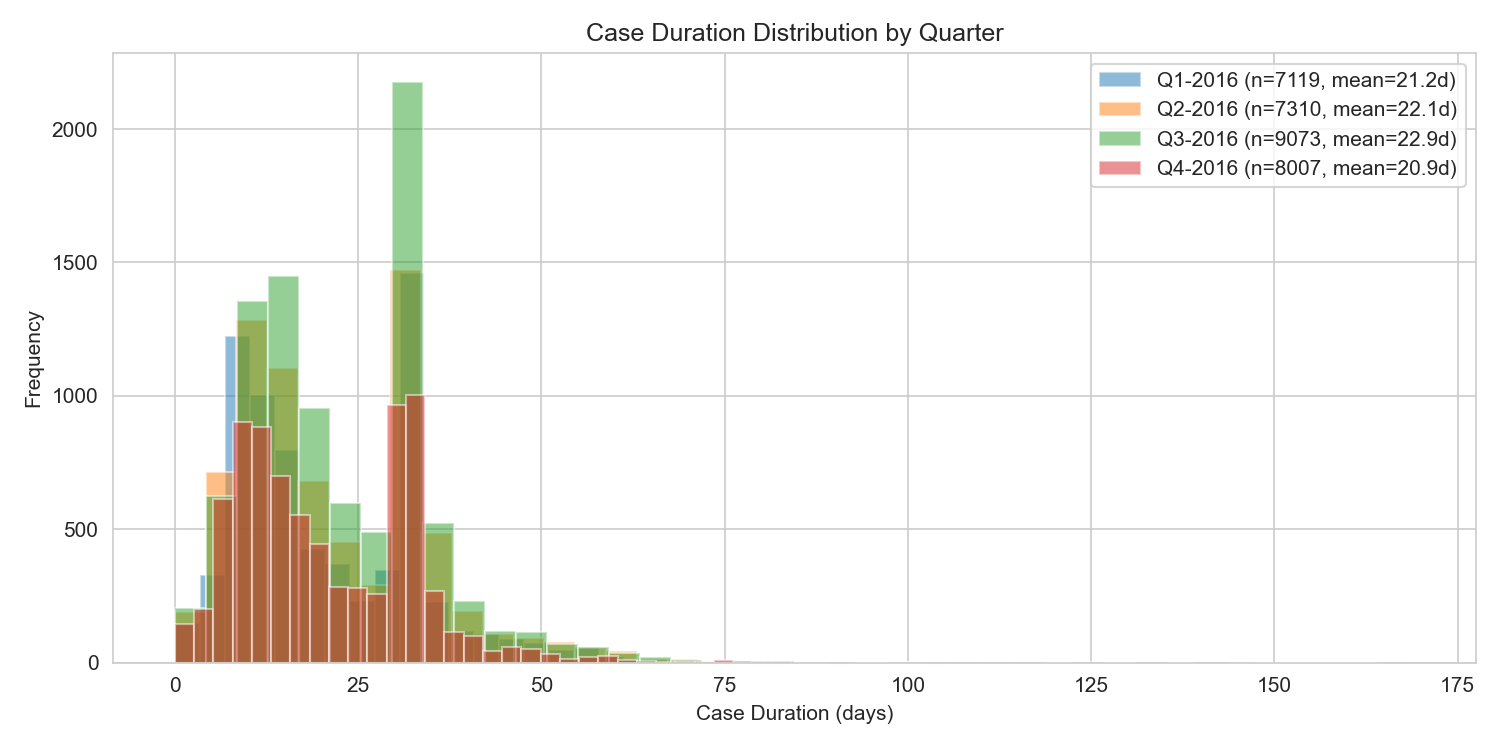
\includegraphics[width=\textwidth]{figures/concept_drift_durations.png}
    \caption{Case duration distributions across the four quarters of 2016. A significant drift is observed ($p < 0.001$).}
    \label{fig:drift_durations}
\end{figure}

\begin{figure}[h]
    \centering
    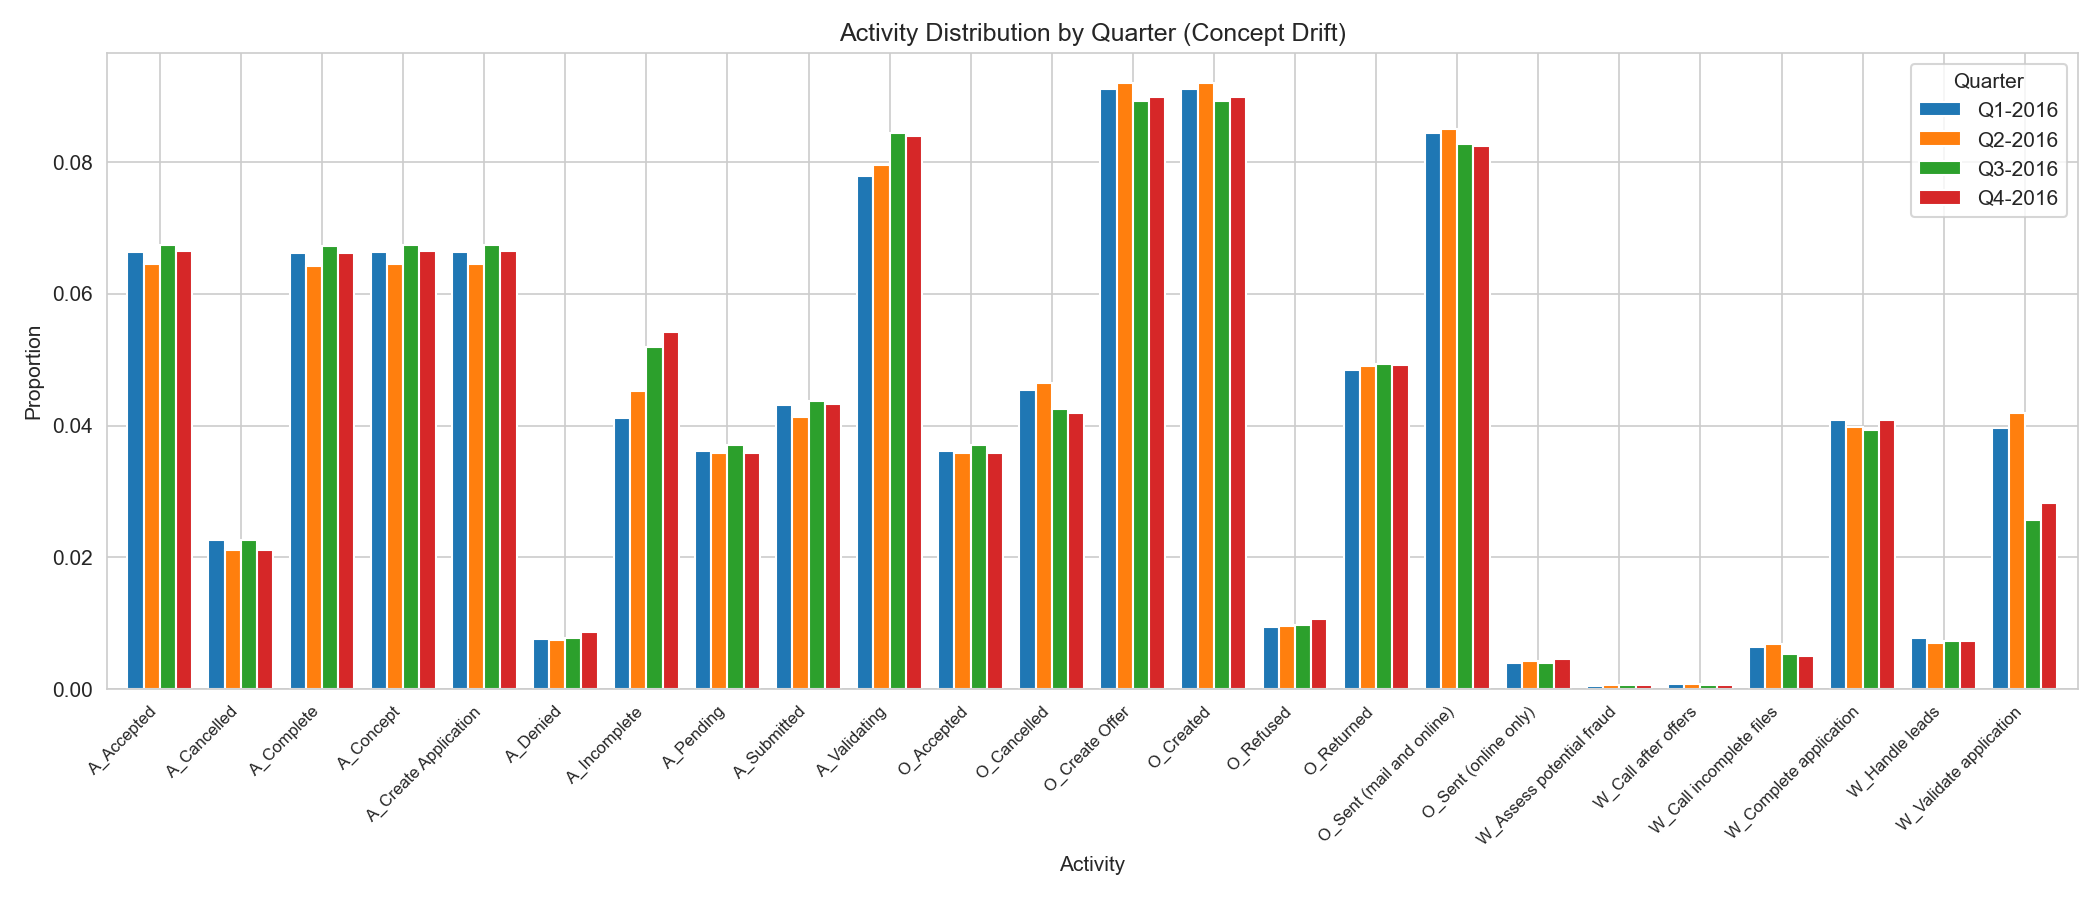
\includegraphics[width=\textwidth]{figures/concept_drift_activities.png}
    \caption{Activity frequency distributions comparing the first and fourth quarters of 2016. The relative frequencies change significantly ($p < 0.001$).}
    \label{fig:drift_activities}
\end{figure}

\begin{figure}[h]
    \centering
    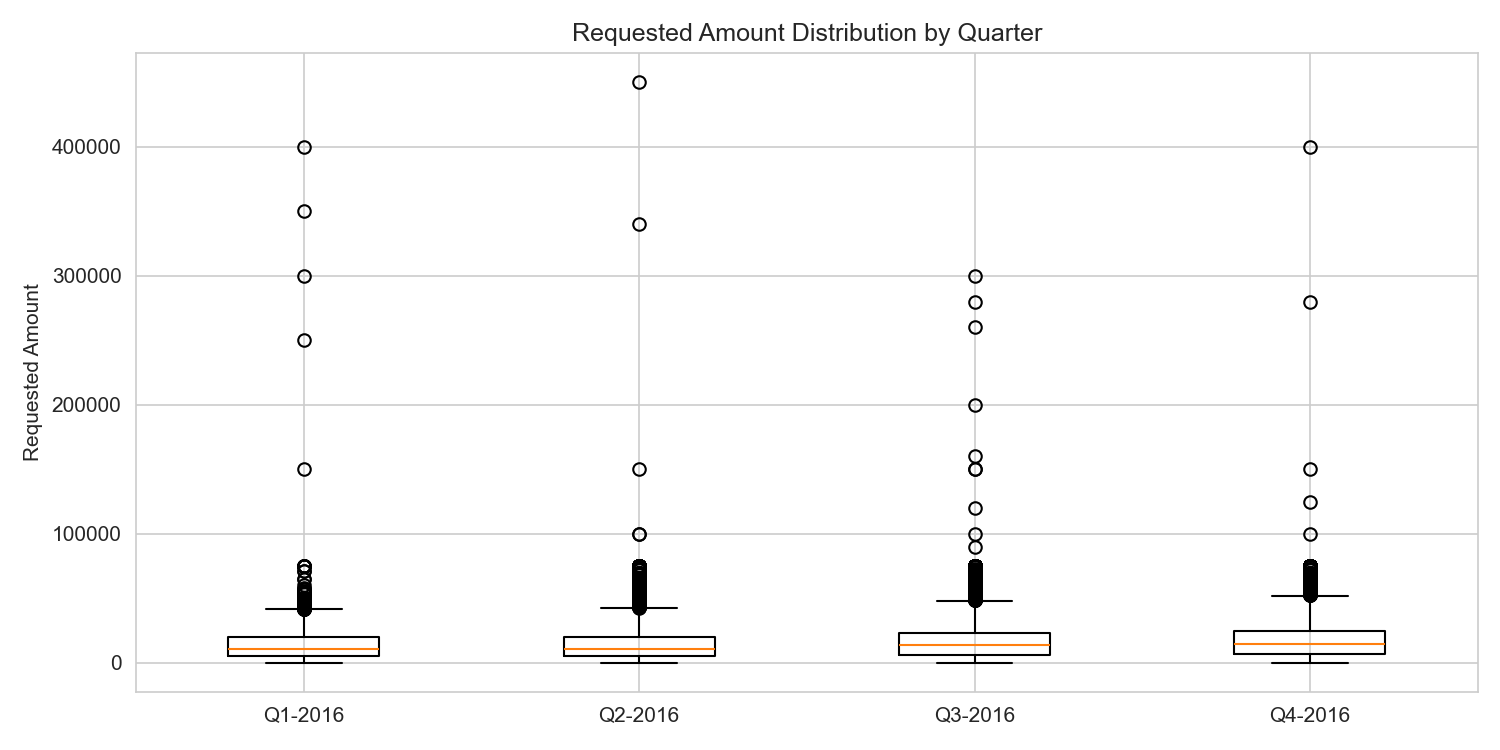
\includegraphics[width=\textwidth]{figures/concept_drift_amount.png}
    \caption{Requested loan amount distributions across the four quarters of 2016. Significant drift is observed ($p < 0.001$).}
    \label{fig:drift_amounts}
\end{figure}

\end{document}
